Während es im Gleichstromkreis nur den Ohm'schen Widerstand gibt, verfügt man im Wechselstromkreis über drei Typen.

Die restlichen zwei Arten, der kapazitive und der induktive Widerstand, generieren Phasenverschiebungen, welche in sogenannten Blindwiderständen resultieren.


\subsection{Ohm'sche Widerstände}		\label{subsec:OhmscherWiderstand}

Wenn in einem Wechselstromkreis nur Ohm'sche Widerstände verbaut sind, ist die Impedanz $Z$, also der Gesamtwiderstand des Kreises, gleich der Summe der Widerstände.

Das bedeutet, er verursacht keine Phasenverschiebung und kann wie ein Widerstand im Gleichstromkreises behandelt werden.


\subsection{Kapazitive Widerstände}		\label{subsec:KapazitiverWiderstand}

Kondensatoren verursachen kapazitive Widerstände. Da Kondensatoren keinen Durchfluss erlauben, wäre ihr Widerstand im Gleichstromkreis unendlich. Im Wechselstromkreis verursacht er aber eine Phasenverschiebung des Stromes, welcher dann um 90\degree{} der Spannung vorauseilt.

Beim Wechselstrom schwingen die elektrischen Ladungen nämlich hin und her. Ein Kondensator im Wechselstromkreis wird also abwechselnd geladen, wieder entladen und dann anders gepolt geladen. Die Spannung zwischen den Kondensatorplatten baut sich während den Ladevorgängen mit der Zeit auf und erreicht ihr Maximum dann, wenn der Kondensator vollständig aufgeladen und der Stromfluss zum Erliegen gekommen ist. Bei den Entladevorgängen sind die Verhältnisse umgekehrt: Die Stromstärke ist dann am größten, wenn der Kondensator vollständig entladen ist.\endnote{Paragraph von: \url{http://files.sma.de/dl/10040/BLINDLEISTUNG-ADE094210.pdf}}

\glqq Der Strom eilt der Spannung voraus.\grqq

\vspace{11pt}

\noindent Dieser sogenannte \glqq Kapazitive Blindwiderstand\grqq{} ist antiproportional abhängig von der Kapazität des Kondensators, da der Anteil der Zeit, in der der Kondensator vollständig oder annähern vollständig geladen ist, größer ist, da eine kleinere Kapazität dafür sorgt, dass mit weniger Ladung schon eine hohe Spannung erreicht wird (Siehe: \gleichungsreferenz{eq:kapazitaet}). Damit ist der Stromfluss bei einer kleinen Kapazität stärker gehemmt als bei einer großen Kapazität. 

$X_C$ ist außerdem antiproportional abhängig von der Winkelgeschwindigkeit (Siehe: \referenz{subsec:ErlaeuterungenGrundlegend}), da bei einer raschen Umpolung der Wechselspannung (also $f$ und demnach auch $\omega$ recht groß) die Zeit in der der Stromfluss durch einen vollständig geladenen Kondensator gehemmt ist, kleiner wird.

Daraus folgt:

\begin{equation}	\label{eq:KapazitiverWiderstand}
	X_C = \frac{1}{\omega \cdot C}
\end{equation}


\subsection{Induktive Widerstände}		\label{subsec:InduktiverWiderstand}

Eine Spule leitet Gleichstrom wie ein normaler Draht. Nur beim Ein- und Ausschalten gibt es jeweils eine Zeitverzögerung im Stromfluss, die durch die Selbstinduktion (Siehe \referenz{sec:Selbstinduktion}) während des Auf- und Abbaus des Magnetfeldes verursacht wird. Unter Wechselstrombedingungen kommt es bei jedem Wechsel der Stromrichtung zu diesen Verzögerungen. Dies resultiert in einer Phasenverschiebung des Stromes um -90\degree .\footnote{Paragraph von: \url{http://files.sma.de/dl/10040/BLINDLEISTUNG-ADE094210.pdf}}

\glqq Die Spannung eilt dem Strom voraus.\grqq

\vspace{11pt}

Der \glqq Induktive Widerstand\grqq{} ist proportional abhängig von der Induktivität der Spule, da ein höheres Vermögen, bei jedem Umpolen Spannung in sich selbst zu induzieren, sich in einer stärkeren Hemmung des Stromflusses äußert.

Der induktive Widerstand ist ebenfalls proportional zur Winkelgeschwindigkeit, da bei einer höheren Winkelgeschwindigkeit öfters umgepolt wird und der Prozess der Selbstinduktion häufiger den Stromfluss hemmt und die Zeit in der der Strom ungehindert fließen kann (nach vollständigem Aufbau des Magnetfeldes) kürzer wird.

Daraus folgt:

\begin{equation}	\label{eq:InduktiverWiderstand}
	X_L = \omega \cdot  L
\end{equation}


\subsection{Auswirkungen von Blindwiderständen auf die Stromstärke} \label{subsec:AuswirkungenWiderstand}

Man kann die Gleichung für die Impedanz (Gleichung \ref{eq:Impedanz} auf Seite \pageref{eq:Impedanz}) nach $I$ umstellen, um sich zu verdeutlichen, dass eine erhöhte Impedanz, in welcher der Blindwiderstand steckt, eine niedrigere Stromstärke zur Folge hat, genau wie der Ohm'sche Widerstand im Wechselstromkreis:

\begin{equation}	\label{eq:ImitZ}
	I_{eff}=\frac{U_{eff}}{Z}
\end{equation}


\subsection{Frequenzabhängigkeit}	\label{subsec:Frequenzabhaengigkeit}

Die Größe der Blindwiderstände ist sowohl beim Kondensator als auch bei der Spule abhängig von der Frequenz des Wechselstromes (diese Steckt im $\omega$).

Der kapazitive Blindwiderstand ist antiproportional abhängig (Siehe Gleichung \ref{eq:KapazitiverWiderstand}) von der Frequenz, was bedeutet: \glqq Ein Kondensator erhöht die Impedanz, je niedriger die Frequenz ist.\grqq{} Man sagt auch \glqq High-Pass-Filter\grqq{} oder \glqq Low-Cut-Filter\grqq .

Der induktive Blindwiderstand ist proportional abhängig (Siehe Gleichung \ref{eq:InduktiverWiderstand}) von der Frequenz, was bedeutet: \glqq Eine Spule erhöht die Impedanz, je höher die Frequenz ist.\grqq{} Man sagt auch \glqq Low-Pass-Filter\grqq oder \glqq High-Cut-Filter\grqq .

Diese Eigenschaften macht man sich in der Audiotechnik bei Frequenzweichen oder Equalisern zu Nutze. Siehe auch \referenz{subsec:Siebkreis}.



\subsection{Zeigerdiagramm}	\label{subsec:WiderstaendeZeigerdiagram}

Die Impedanz ist auch berechenbar, wenn der Ohm'sche Widerstand und der Blindwiderstand bekannt sind. Bevor Gesetze betrachtet werden, ist das Zeigerdiagramm\endnote{"Zeigerdiagramm für Widerstände" by Till Blaha - Mit Gnuplot selbst erstellt. Lizenziert unter Gemeinfrei.} eine gute Veranschaulichung für die Beziehungen und den Phasenverschiebungswinkel.

\begin{figure}[h!]
	\centering
	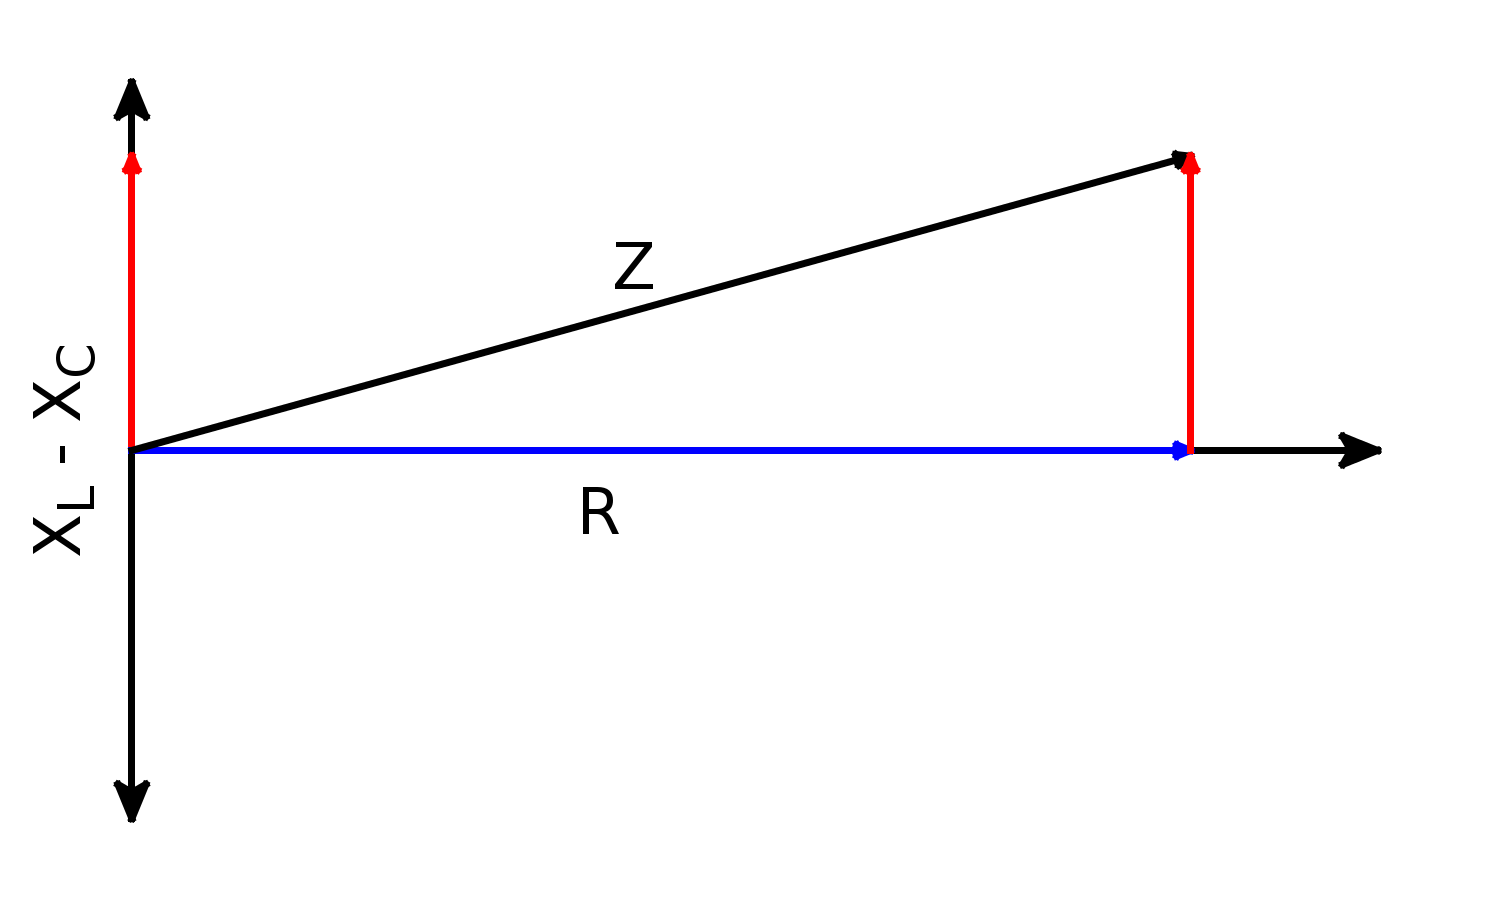
\includegraphics[width=0.8\textwidth]{plot_zeigerdiagramm}
	\begin{comment} Gnuplot:
set ylabel "X_L - X_C"
set label "R" at 2.5,-0.2
set label "Z" at 2.7,0.6
set arrow from graph 0,0.5 to graph 0,0.9 size screen 0.01,22,60 filled ls 1 front
set arrow from graph 0,0.5 to graph 0.85,0.5 size screen 0.01,22,60 filled ls 3 front
set arrow from graph 0,0.5 to graph 0.85,0.9 size screen 0.01,22,60 filled ls 2 front
set arrow from graph 0.85,0.5 to graph 0.85,0.9 size screen 0.01,22,60 filled ls 1 front
unset key
set output "plot_zeigerdiagramm.png"
plot 100
	\end{comment}
	\caption{Zeigerdiagramm mit Widerständen: Blau: Ohm'scher Widerstand, Rot: Blindwiderstand, Schwarz: Impedanz, Der Phasenverschiebungswinkel ist der Winkel zwischen der Impedanz (Hypothenuse) und dem Ohm'schen Widerstand (Kathete)}
\end{figure}


Das Diagramm veranschaulicht den Zusammenhang zwischen dem Verhältnis des Blindwiderstandes und dem Ohm'schen Widerstand. Dieses Verhältnis ist nämlich immer gleich dem Tangens des Winkels $\varphi$.

\begin{Anmerkung}
Sollten in einem Schaltkreis beide Blindwiderstände (eine Spule und ein Kondensator) verbaut sein, muss für die Differenz für $X_{Ges}$ angenommen werden, da beide eine Phasenverschiebung in die jeweils andere Richtung verursachen.
\end{Anmerkung}

\noindent Für $X_{Ges}$ gilt dann:

\begin{equation}	\label{eq:BlindwiderstandSumme}
	X_{ges} = X_L - X_C = \omega \cdot L - \frac{1}{\omega \cdot C}
\end{equation}



\subsection{Gesetze}	\label{subsec:WiderstaendeGesetzte}

Nun ist auch die Betrachtung der Gesetze, angelehnt an diese Darstellungsform, deutlich einfacher.


Für die Impedanz können nun, zusätzlich zur \gleichungsreferenz{eq:Impedanz}, noch andere Betrachtungen gefunden werden:

In Abhängigkeit von $X$ und $R$ mit dem Satz des Pythagoras:

\begin{equation}	\label{eq:ImepdanzXR}
	Z = \sqrt{X^2 + R^2}
\end{equation}


\noindent In Abhängigkeit von $X$ und $\varphi$ mit weiteren Winkelbeziehungen im rechtwinkligen Dreieck:

\begin{equation}	\label{eq:ImepdanzXphi}
	Z = \frac{X}{\sin\varphi}
\end{equation}


\noindent In Abhängigkeit von $R$ und $\varphi$:

\begin{equation}	\label{eq:ImepdanzRphi}
	Z = \frac{R}{\cos\varphi}
\end{equation}